\documentclass[10pt]{beamer}

\usetheme{metropolis}
\usepackage{appendixnumberbeamer}


\usepackage{booktabs}
\usepackage[scale=2]{ccicons}

\usepackage{pgfplots}
\usepgfplotslibrary{dateplot}


\usepackage{amsmath}
\usepackage{media9}
\usepackage{xspace}
\usepackage{xcolor}
\usepackage{tikz}
\usetikzlibrary{bayesnet} %for plate notation
\usepackage{listings} %for printing python code


%%%% This next section builds the \warning symbol
\usepackage[utf8]{inputenc}
\usepackage{xcolor}
\usepackage{newunicodechar}

\newcommand\warning{%
 \makebox[1.4em][c]{%
 \makebox[0pt][c]{\raisebox{.1em}{\small!}}%
 \makebox[0pt][c]{\color{red}\Large$\bigtriangleup$}}}%
 

\usepackage[most]{tcolorbox} %for color box
%Reference:
% 	https://tex.stackexchange.com/questions/279464/2-boxed-equations-on-one-lineblue-outline-box-and-shadow
%Usage:
%	\tcboxmath{something}


%https://tex.stackexchange.com/questions/395140/change-font-size-of-one-equation-in-align-environment?rq=1
%has medmath for reducing font size in align environments
\usepackage{mathtools, nccmath} 


%https://jansoehlke.com/2010/06/strikethrough-in-latex/
%lets you cancel out terms in an equation
\usepackage{cancel}

\newcommand{\themename}{\textbf{\textsc{metropolis}}\xspace}

% THEOREM STYLES 
% Reference: https://www.overleaf.com/learn/latex/Theorems_and_proofs
\usepackage{amsthm}
\numberwithin{equation}{section}

%\newtheorem{theorem}{Theorem}[section]
\newtheorem{proposition}[theorem]{Proposition}
%\newtheorem{lemma}[theorem]{Lemma}
%\newtheorem{corollary}[theorem]{Corollary}
%\newtheorem{conjecture}[theorem]{Conjecture}
%\newtheorem{question}[theorem]{Question}




\theoremstyle{definition}
%\newtheorem{definition}[theorem]{Definition}
%\newtheorem{property}[theorem]{Property}
%\newtheorem{notation}[theorem]{Notation}
%\newtheorem{exercise}[theorem]{Exercise}
%\newtheorem{problem}[theorem]{Problem}
\newtheorem{claim}[theorem]{Claim}
%\newtheorem{remark}[theorem]{Remark}
%%% Reference on example as environment: https://tex.stackexchange.com/questions/21227/example-environment
%\newtheorem{example}[theorem]{Example}

%%% GENERALLY USEFUL 
\newcommand{\ds}{\displaystyle}
\newcommand{\df}{\displaystyle\frac}
\newcommand{\R}{\mathbb{R}}
\newcommand{\+}[1]{\ensuremath{{\boldsymbol #1}}} %another way to make bold symbols
\newcommand{\cond}{\; | \;}
\newcommand{\blue}[1]{\color{blue}{#1}  \color{black}}
\newcommand{\red}[1]{\color{red}{#1}  \color{black}}
\newcommand{\green}[1]{\color{green}{#1}  \color{black}}
\newcommand{\purple}[1]{\color{purple}{#1}  \color{black}}
\DeclareMathOperator*{\argmax}{argmax} % thin space, limits underneath in displays
\newcommand{\partialderiv}[2]{\df {\partial {#1}}{\partial {#2}} }
\newcommand{\biggexp}[1]{\exp  \bigg\{ {#1} \bigg\} }


%%% PROBABILITY
\newcommand{\iid}{\stackrel{\text{iid}}{\sim}}
\newcommand{\norm}{\mathcal{N}}
\newcommand{\IG}{\mathcal{I}\mathcal{G}}
\newcommand{\E}{\mathbb{E}}
\newcommand{\biggE}[2]{\E_{{#1}} \bigg[ {{#2}} \bigg]}
%\newcommand{\H}{\mathbb{H}}
\newcommand{\Prob}{\mathbb{P}}
\newcommand{\absdet}[1]{ \; \bigg\lvert \det{#1}  \bigg\rvert  \;}
\newcommand{\logabsdet}[1]{ \log \absdet{#1}}
\newcommand{\KL}[2] {\texttt{KL} \big({#1} \; \big|\big| \; {#2} \big)}
\newcommand{\Q}{\mathcal{Q}}
\newcommand{\ind}{\perp\kern-5pt\perp}

%%% INTEGRALS
\newcommand{\wrt}[1]{\; d \,{#1} \;} 

%%% SETS
\newcommand{\set}[1] { \{  {#1} \} }
\newcommand{\cupdot}{\sqcup}


%%%% TYPEWRITER FONTTED VI ACRONYMS 
\newcommand{\bbvi}{\,\texttt{bbvi}\,}
\newcommand{\VLBO}{\,\texttt{VLBO}\,}
\newcommand{\ELBO}{\,\texttt{ELBO}\,}

%% SHADED BOXES
%colored shaded boxes
\newcommand{\bluebox}[2] { \tikz[baseline]{\node[fill=blue!20,anchor=base]({#1}) { {#2} } }}
\newcommand{\redbox}[2] { \tikz[baseline]{\node[fill=red!20,anchor=base]({#1}) { {#2} } }}
\newcommand{\greenbox}[2] { \tikz[baseline]{\node[fill=green!20,anchor=base]({#1}) { {#2} } }}
%these put a label beneath the shaded box, in the same color
\newcommand{\labeledbluebox}[2]{  \underset{\blue{#1}}{\bluebox{_dummy_}{#2}} }
\newcommand{\labeledredbox}[2]{  \underset{\red{#1}}{\redbox{_dummy_}{#2}} }
\newcommand{\labeledgreenbox}[2]{  \underset{\green{#1}}{\greenbox{_dummy_}{#2}} }
%https://github.com/matze/mtheme

%% CHECKMARK 
\usepackage{pifont}% for cmark and xmark for checkmark and xmark 
\newcommand{\cmark}{\ding{51}}%
\newcommand{\xmark}{\ding{55}}%
\newcommand{\greencheck}{\green{\cmark}}
\newcommand{\redx}{\red{\xmark}}

%%% EXPLANATIONS  
%explaining equations 
\newcommand{\explaineq}[1]{\stackrel{\text{#1}}{=}}
%explain terms
\newcommand{\explainterm}[2]{\underset{\textit{#1}}{#2}}
%explain terms with underbrace
\newcommand{\explaintermbrace}[2]{\underbrace{#2}_{\text{#1}}}



%\title{Variational Inference: A Historical Perspective}
\title{Fitting Gaussian Mixture Models with Variational Inference}
%\subtitle{With Application To General Deobfuscation of Windows API Calls}
%\subtitle{Part 1: Foundations}
%\date{\today}
\author{Michael Thomas Wojnowicz}
%\institute{Data Intensive Studies Center, Tufts University}
%\titlegraphic{\hfill\includegraphics[height=1.5cm]{logo.pdf}}


%TO DRAW ARROWS WITH EQUATIONS AND SHADE THEM.
% REFRENCE: http://www.texample.net/tikz/examples/beamer-arrows/
% For every picture that defines or uses external nodes, you'll have to
% apply the 'remember picture' style. To avoid some typing, we'll apply
% the style to all pictures.
\tikzstyle{every picture}+=[remember picture]

%\AtBeginSubsection{\frame{\subsectionpage}}

\begin{document}

\maketitle

\begin{frame}{Table of contents}
  \setbeamertemplate{section in toc}[sections numbered]
  \tableofcontents[hideallsubsections]
\end{frame}


\section{Variational Inference: Overview}



%%%%%%%%%%%%%%%%%%%%%%%%%%%%%%%%%%%%%%%%%%%%%%%%%%
\begin{frame}{Illustration}

 \begin{minipage}[t][.9\textheight]{\textwidth}
  
Here we approximate an probability density by finding the best approximation from tractable family $\Q = \{ \text{10-component Gaussian mixture models} \}$ 

\begin{columns}[t]
\column{.5\textwidth}
\centering
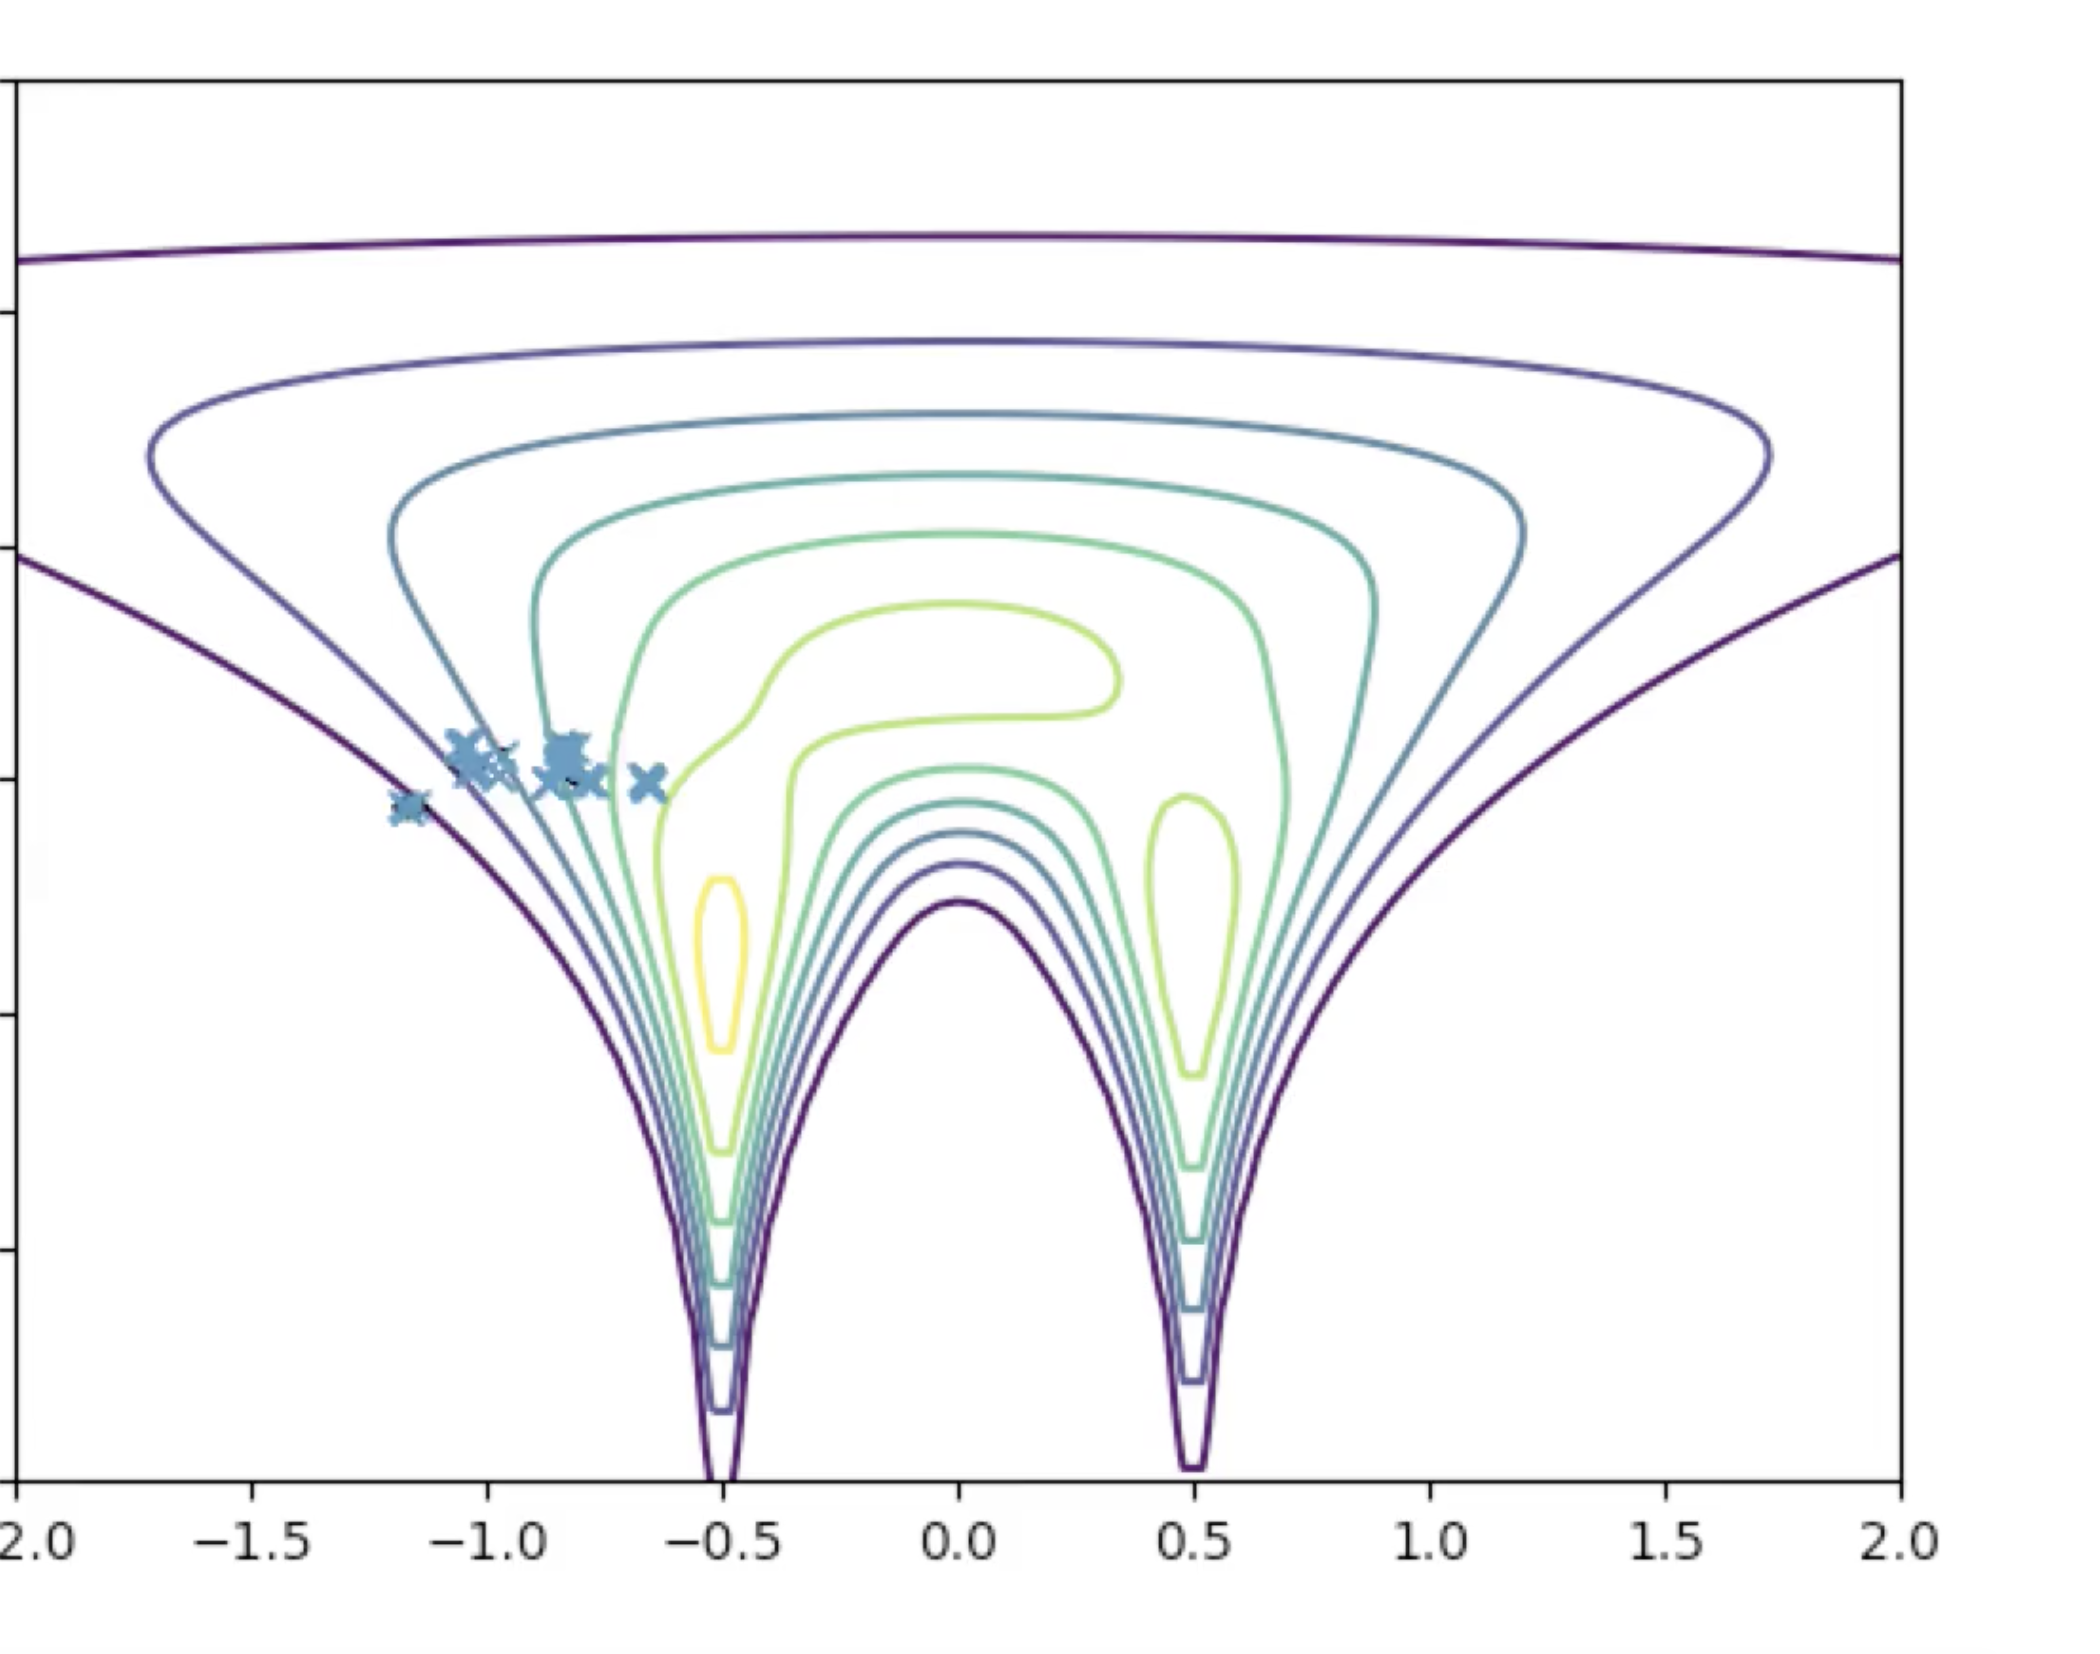
\includegraphics[width=.7\textwidth]{images/intro_animation_1.png}\\
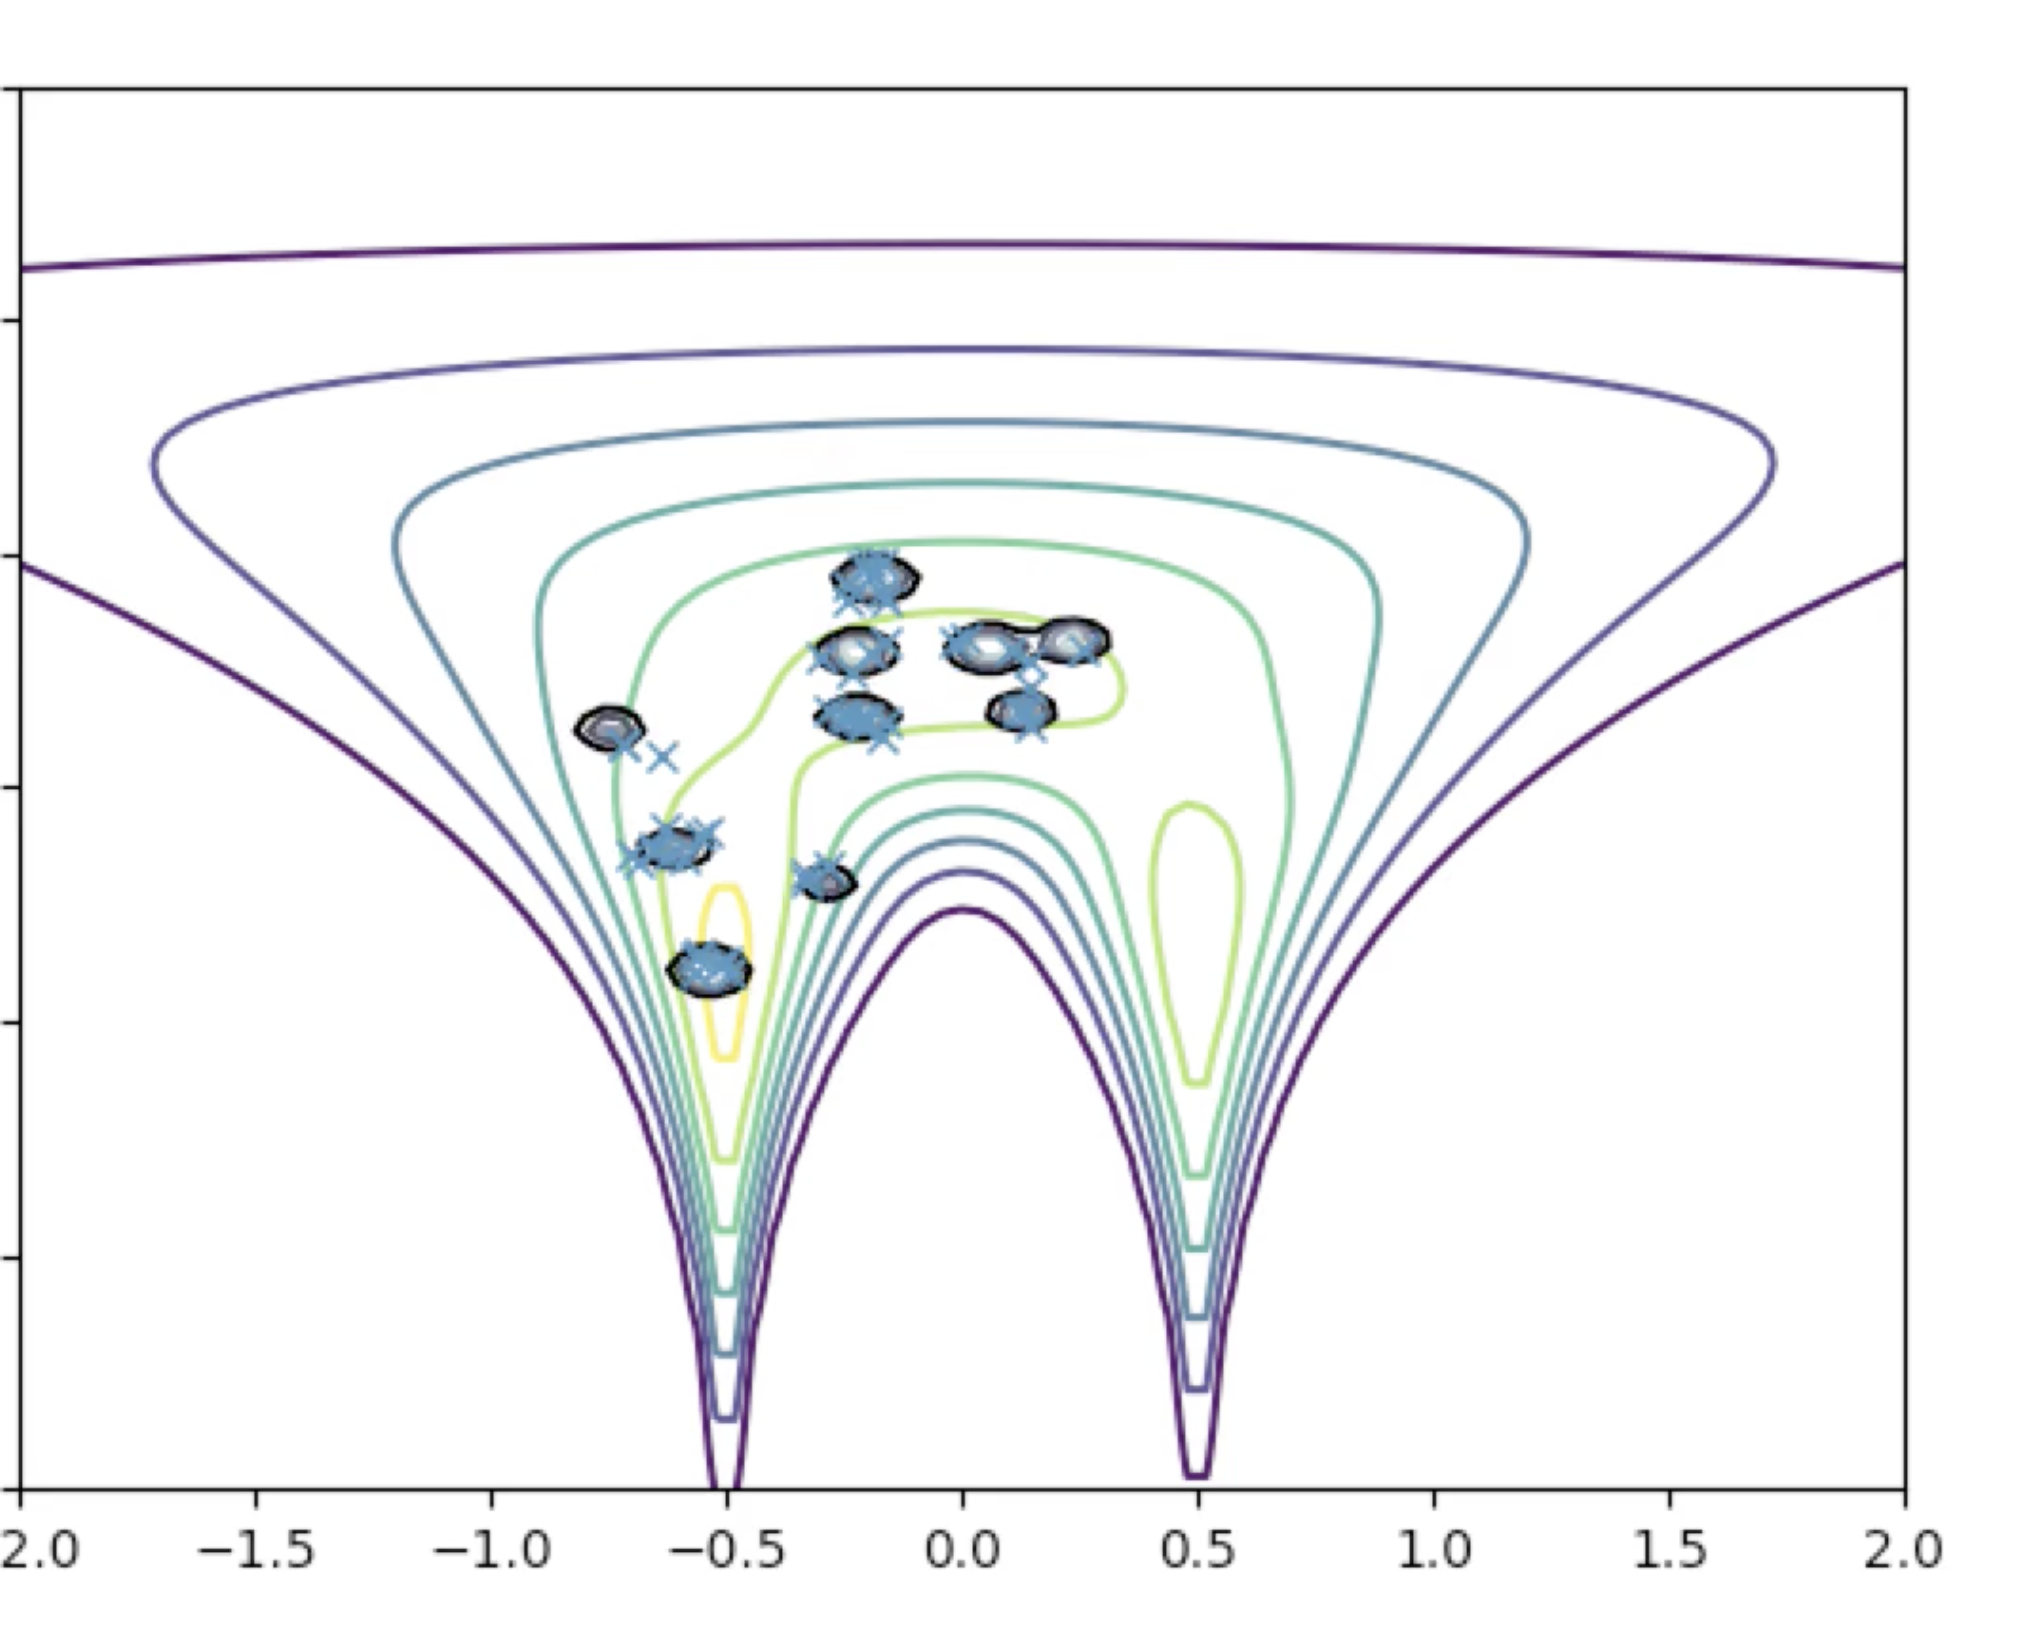
\includegraphics[width=.7\textwidth]{images/intro_animation_2.png}
\column{.5\textwidth}
\centering
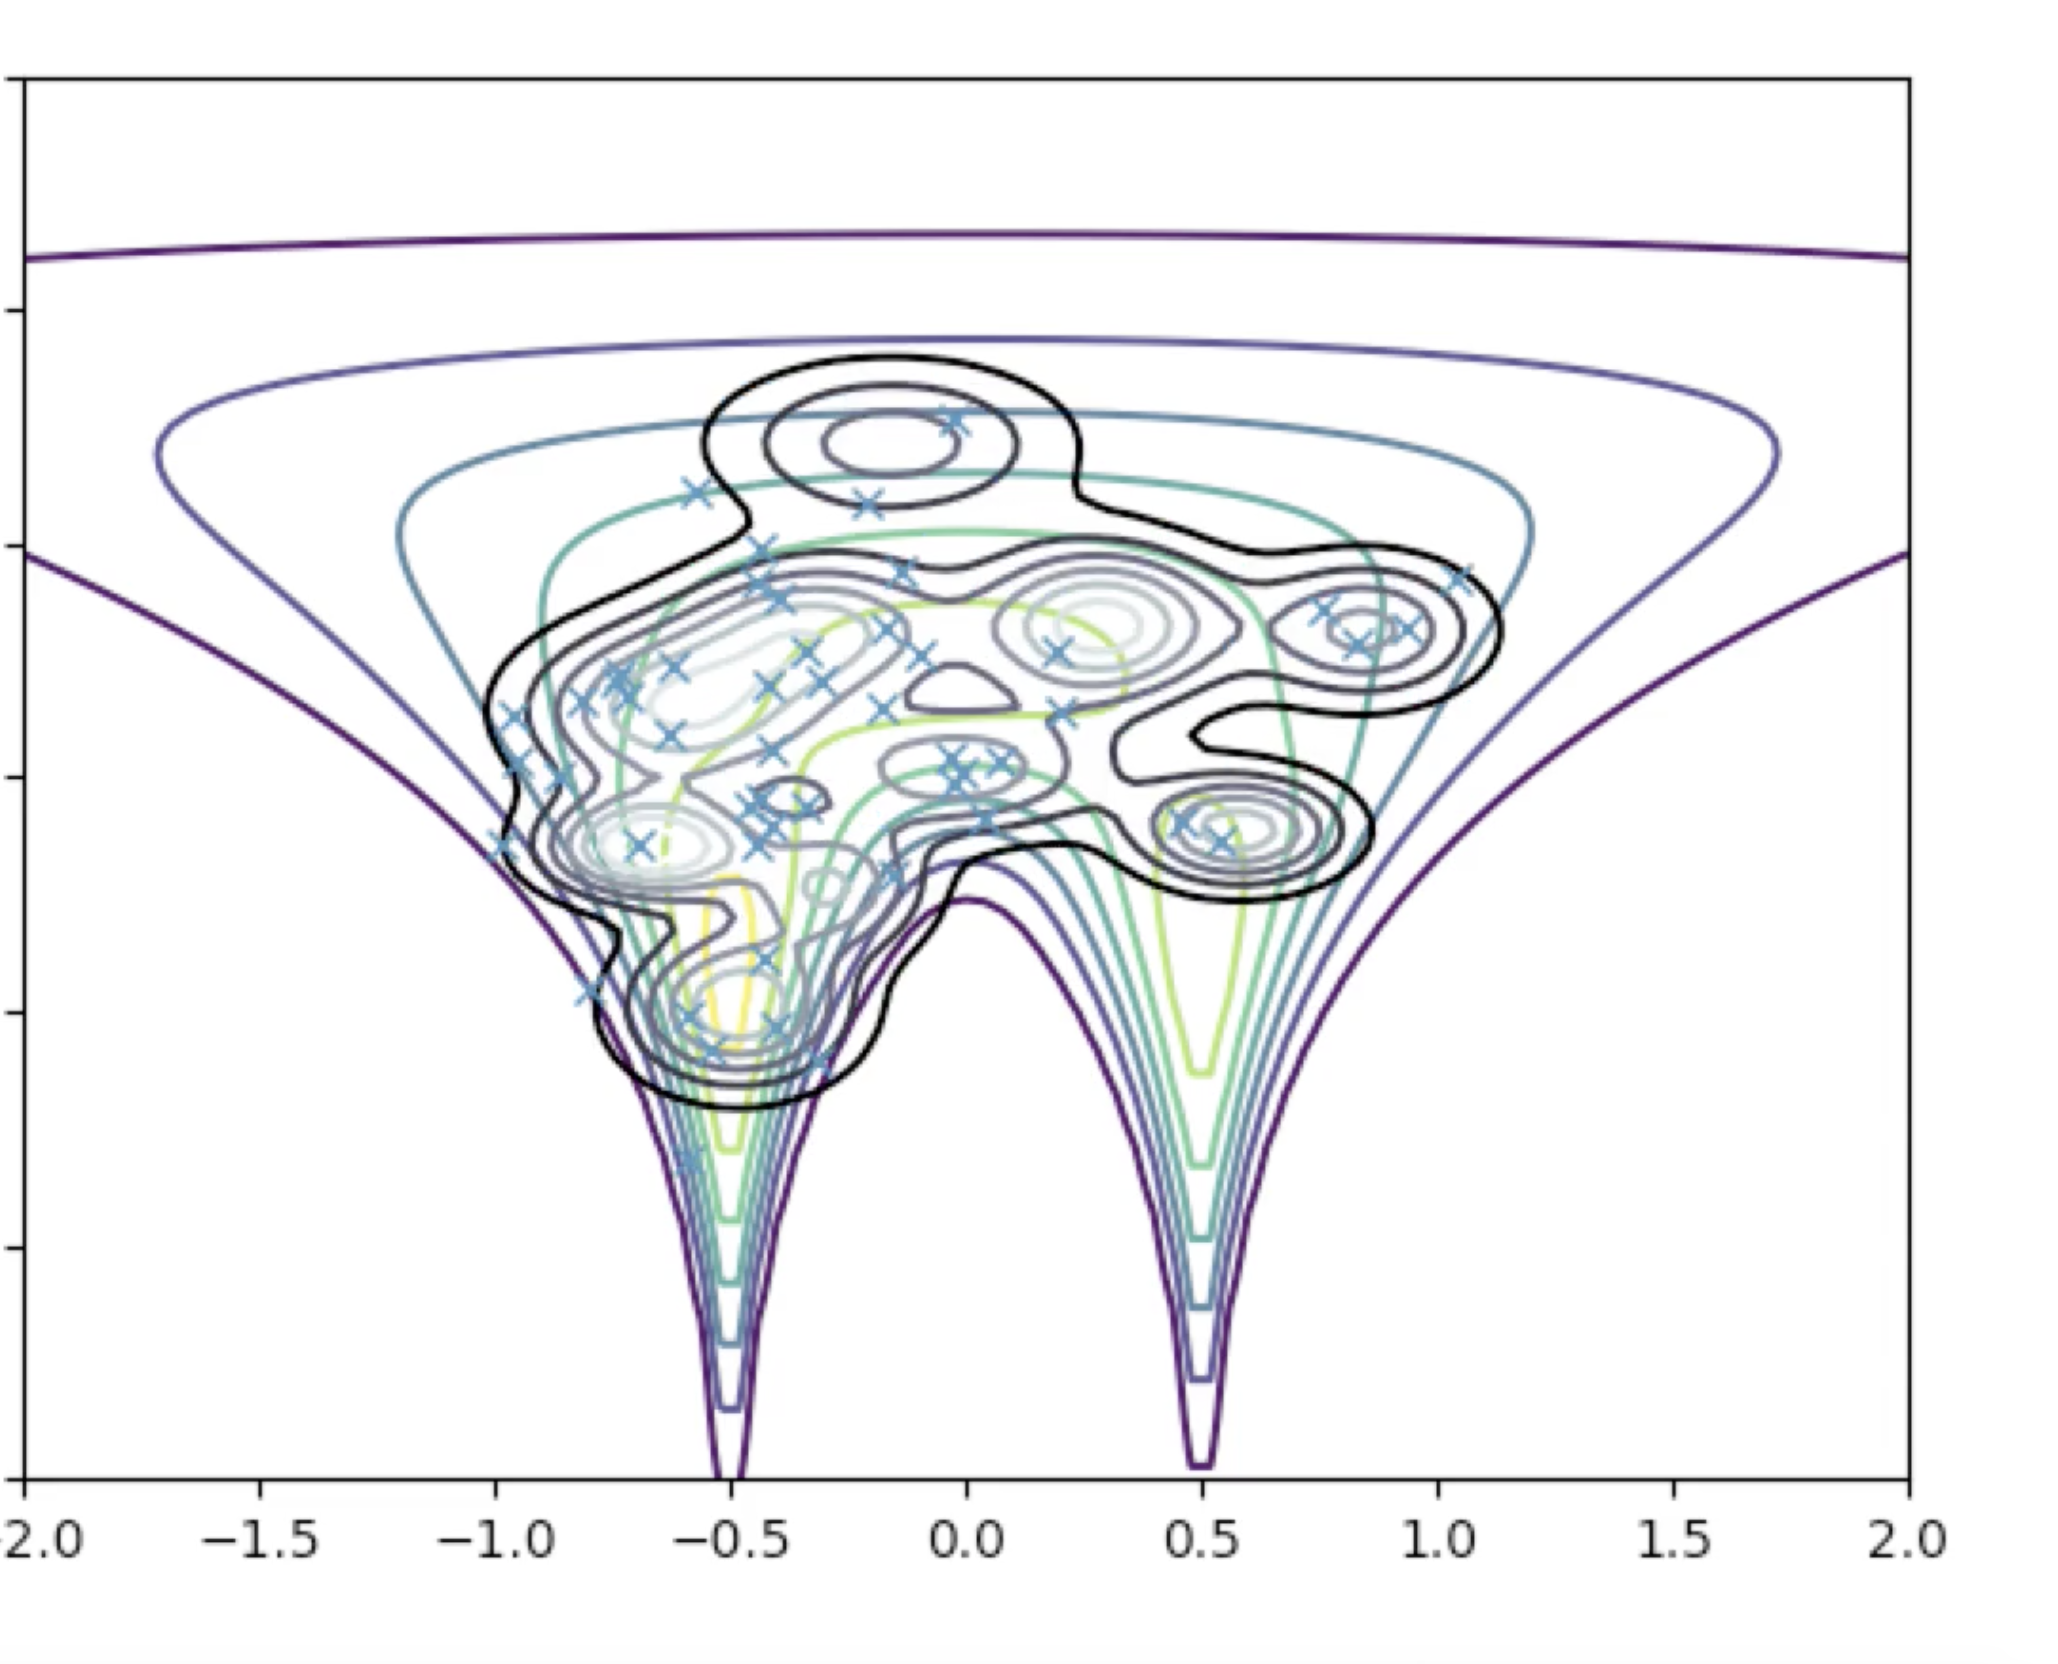
\includegraphics[width=.7\textwidth]{images/intro_animation_3.png}\\
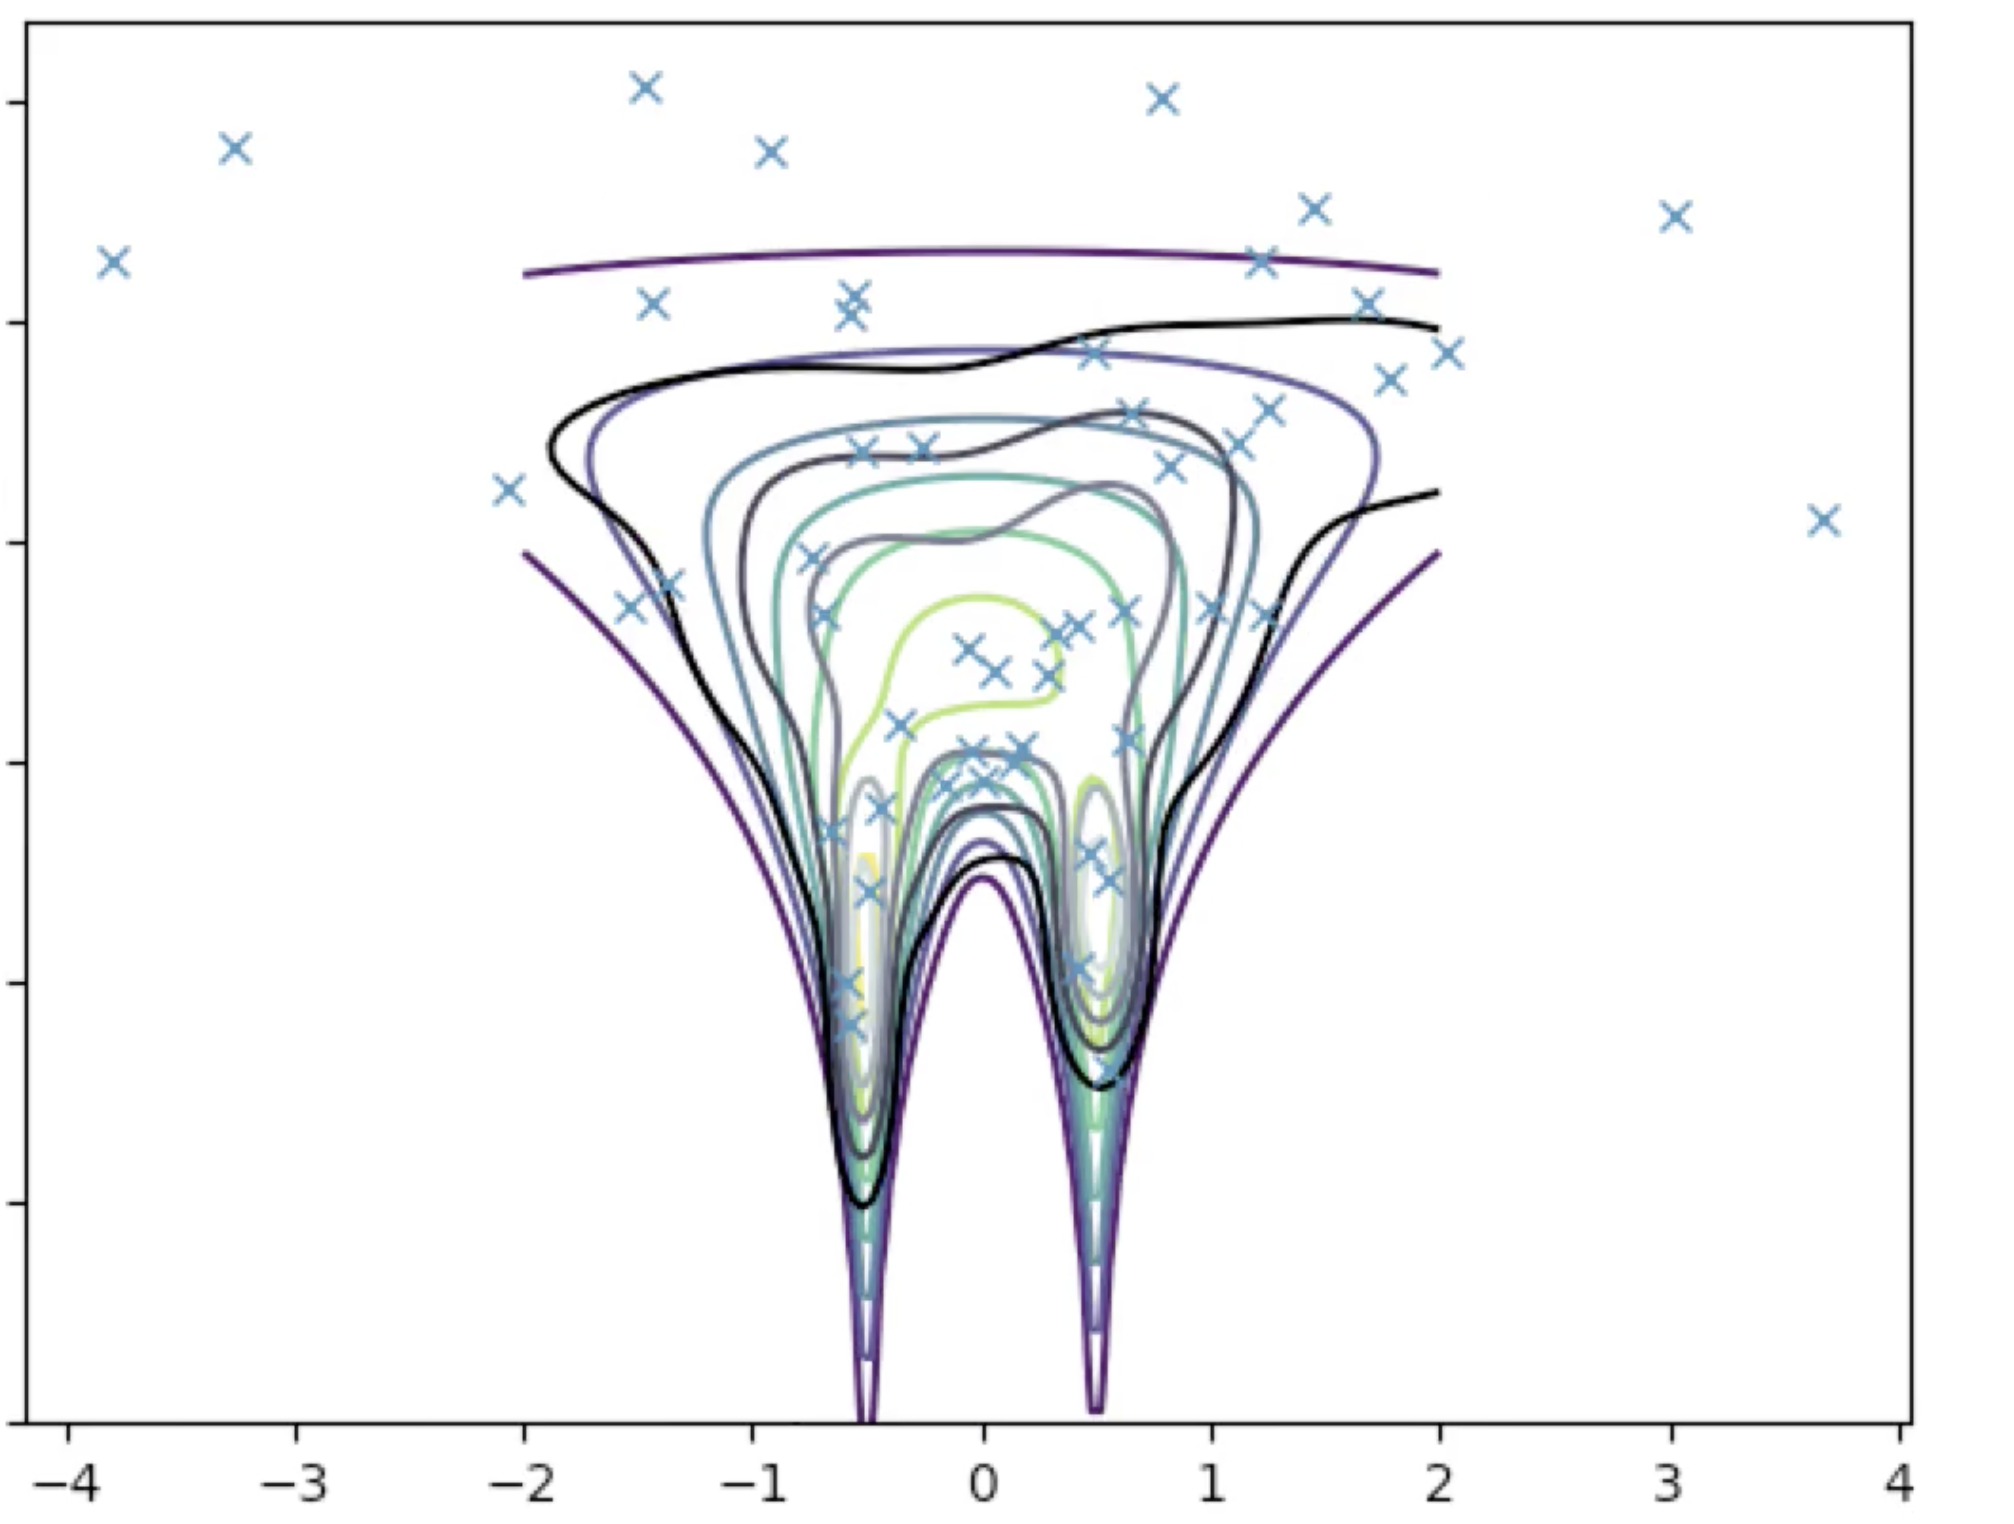
\includegraphics[width=.7\textwidth]{images/intro_animation_4.png}
\end{columns}

\vfill

%\tiny Ranganath, R., Gerrish, S., \& Blei, D. (2014, April). Black box variational inference. In Artificial Intelligence and Statistics (pp. 814-822).
  \end{minipage}
  
\end{frame}


%%%%%%%%%%%%%%%%%%%%%%%%%%%%%%%%%%%%%%%%%%%%%%%%%%
\begin{frame}{Statistical inference in Bayesian models}


\metroset{block=fill}
\begin{block}{}

By Bayes' rule, we cannot get the posterior without the \textbf{evidence}
\begin{equation}
p(\+x) =  \ds\int p(\+x,\+u) \wrt{\+u}
\end{equation}

where 
\begin{itemize}
\item $\+x$: observed data 
\item $\+u$: unobserved random variables
\end{itemize}

\end{block}

\end{frame}


%%%%%%%%%%%%%%%%%%%%%%%%%%%%%%%%%%%%%%%%%%%%%%%%%%
\begin{frame}{How variational inference works}
 

We construct a lower bound on the evidence. 

\metroset{block=fill}
\begin{block}{Evidence Lower Bound (ELBO)}
Let $q$ be any probability density over $\+u$. Then:

\begin{align*}
\ln p(\+x) & = \ln \ds\int  p(\+u, \+x) \wrt{\+u}  \\ 
& = \ln \ds\int  q(\+u) \; \df{p(\+u, \+x  )}{q(\+u)} \wrt{\+u}  \\ 
& \stackrel{Jensen's}{\geq} \ds\int  q(\+u) \; \ln \bigg( \df{p(\+u, \+x)}{q(\+u)} \bigg) \wrt{\+u} \\
& : = \ELBO(q) 
\end{align*}
\end{block} 

We want to find $q \in \mathcal{Q}$ to maximize the $\ELBO$.
 

\end{frame} 
%


%%%%%%%%%%%%%%%%%%%%%%%%%%%%%%%%%%%%%%%%%%%%%%%%%%%
\begin{frame}{What maximizes the \ELBO \\ also minimizes the KL divergence to the posterior}  

%The variational density $q \in \mathcal{Q}$  which maximizes the \VLBO also minimizes the KL divergence from the target posterior $p(\+u \cond \+x, \+c)$ %to the variational density. 

By definition, the \texttt{KL} divergence from the target posterior to the variational density is given by
\begin{equation*}
\texttt{KL} (q(\+u) \; || \; p(\+u \cond \+x)) =  \E_q \bigg[\log \df{q(\+u )}{p(\+u \cond \+x)} \bigg] 
\end{equation*}

 

%\begin{equation*}
% \texttt{KL} (q(\+u) \; || \; p(\+u \cond \+x, \+c)) =  \E_q[\log q(\+u )]  - \E_q[ \log p(\+u \cond \+x, \+c)] 
%\end{equation*}

By the chain rule, we get 
\begin{align*} 
 \texttt{KL} (q(\+u) \; || \; p(\+u \cond \+x)) & =  \E_q[\log q(\+u )]  - \E_q[ \log p(\+x,\+u )] &&+\log p(\+x) \\
 & = \hphantom{blah} -\ELBO(q)  && +  \text{constant} 
 \end{align*}
 
%Note that the term $p(\+x \cond \+c)$, is constant in the minimization.  Thus, we may equivalently maximize the negative of the first two terms, which is the \VLBO.

 
%\pause
%\alert{Note}: The optimal variational density, $q^*(\+u)$ is the target posterior density $p(\+u \cond \+x, \+c)$ when the underlying variational family $\Q$ is unrestricted  


\end{frame}


\begin{frame}{Mean Field Coordinate Ascent Variational Inference (MF-CAVI)}

\metroset{block=fill}
\begin{block}{Mean field variational families}
A variational family $\Q$ is mean field if it factorizes 

\begin{equation} \label{mean_field}
q(u_1, ..., u_K) = \ds\prod_{k=1}^K q_k(u_k)
\end{equation}
\end{block}

\textit{Mean field coordinate ascent variational inference (MF-CAVI)} iteratively optimizes each variational density, while holding the others fixed. \\
\vfill
 \tiny \alert{Note}: Since the \ELBO maps probability densities to a real number, it is a functional, so such optimization can be handled with variational calculus.   
   
\end{frame}

\begin{frame}{Update equations for MF-CAVI}

Given the mean field assumption \eqref{mean_field}, the optimal updates to $\set{q_k}_k$ for coordinate ascent on the \ELBO satisfy 
 
\begin{equation} \label{mfcavi_update}
q_k(u_k) \propto \exp \bigg\{ \E_{q_{-k}} \bigg[  \log p(\+u, \+x)\bigg] \bigg\}
\end{equation}

%\vfill
%\tiny
%\alert{Note:} The argument to the expectation, known as the \textit{complete conditional}, is what is used in Gibbs sampling.  % So instead of iteratively sampling from the complete conditionals, we take variational expectations with respect to the same distributions.
%
%%\pause
%
%\alert{Note:} Note that the mean-field assumption \eqref{mean_field} is non-parametric (i.e., no assumptions were made about the parametric family to which $q$ belongs).   The derivation of the update equations  \eqref{mfcavi_update} also has this feature.  Hence, these update equations can be used to determine the optimal parametric families for each of the variational factors.  \\


\end{frame}

\section{Example: Bayesian Gaussian Mixture Model}
\begin{frame}{Example: Bayesian Gaussian Mixture Model}

To see the mean field CAVI algorithm \eqref{mfcavi_update} in a concrete context, consider a version of the Bayesian Gaussian Mixture Model.  
\begin{align*}
\mu_k & \sim \text{Normal}(0, \sigma^2) && k = 1,..., K\\
c_i & \sim \text{Categorical}(\pi_1, ..., \pi_K) && i=1, ... ,n \\
x_i \cond c_i, \mu & \sim \text{Normal}(c_i^T \mu, 1) && i = 1,..., n
\end{align*}
\tiny (The model is simple in that it assumes that each mixture component has unit variance.) \normalsize 

The joint density, by chain rule, is
\[ p(x,c,\mu) = p(\mu) \ds\prod_{i=1}^n p(c_i) p(x_i \cond c_i, \mu) \]

And a mean-field variational family is given by 
\[  q(c, \mu) = \ds\prod_{k=1}^K q(\mu_k) \ds\prod_{i=1}^n q(c_i) \]

\end{frame}

\begin{frame}{Example: Bayesian Gaussian Mixture Model}
We apply \eqref{mfcavi_update} to determine the coordinate updates for $q_{c_i}$, the variational factors governing cluster assignments.   We take the log of the joint and discard terms that do not depend upon $c_i$ to obtain

\begin{align*}
q(c_{ik}) & \propto \exp \bigg\{ \E_{q_{\mu_k}} \bigg[  \log p(c_i =k) + \log p(x_i \cond c_i=k, \mu) \bigg] \bigg\} \\
& \propto \exp \bigg\{ \E_{q_{\mu_k}} \bigg[ \log \pi_k + x_i \mu_k - \df{1}{2} \mu_k^2 \bigg] \bigg\} \\
& \propto \pi_k \exp \bigg\{ x_i \E_{q_{\mu_k}} [\mu_k] - \df{1}{2}  \E_{q_{\mu_k}} [ \mu_k^2] \bigg\} \\
\end{align*}

The coordinate updates for $q_{\mu_k}$ are derived similarly.  They reveal that $q_{\mu_k}$ are Gaussian, and hence the above expectations are easy to compute. 

\end{frame}

\section{Appendix} 

\begin{frame}{Bayesian Gaussian Mixture Model: \\ Updates to mixture component means}
Using the same strategy as when updating cluster assignments $c_i$, we obtain

\begin{align*}
q(\mu_k) & \propto \exp \bigg\{ \E_{-q_{\mu_k}} \bigg[  \log p(\mu_k) + \ds\sum_{i=1}^n \log p(x_i \cond c_i=k, \mu) \bigg] \bigg\} \\
& \propto \exp \bigg\{ -\df{1}{2  \sigma^2} \mu_k^2 +  \ds\sum_{i=1}^{n} \E_{q_c} \bigg[ \+1_{c_i=k}\, \bigg(x_i \mu_k - \df{1}{2} \mu_k^2\bigg) \bigg] \bigg\} \\
& \propto \exp \bigg\{ -\df{1}{2} \bigg(\df{1}{ \sigma^2} + \ds\sum_{i=1}^n q(c_{ik}) \bigg) \mu_k^2 \; +  \;  \bigg( \ds\sum_{i=1}^n q(c_{ik})x_i  \bigg) \mu_k \bigg\} \\
\end{align*}

which is an exponential family distribution with sufficient statistics $(\mu_k, \mu_k^2)$, and hence Gaussian.

\end{frame}

\end{document}

